\chapter{Nested Class Modularity in Squeak}
In this chapter, we describe the main concept of our work: classes as class members. Similar concepts are part of programming languages like Java, Ruby, Python, and Newspeak. Our concept follows closely the Newspeak notion of nested classes, but without making invasive changes to the Smalltalk programming language.

\section{Nested Classes}
In Smalltalk, every object is an instance of a class, defining the object's instance variables and the messages it understands. Consequently, a class is also an instance of its so-called meta class. Every meta class is an instance of \texttt{Metaclass}. In the remainder of this work, we denote the meta class of a class \texttt{C} by \texttt{C class}. Every Smalltalk image has a \texttt{globals} dictionary, mapping symbols to class objects, so that references to classes can be resolved at compile time. This implies that all references to classes are early bound.

Our system extends the Smalltalk class organization as follows: in addition to regular methods, we introduce the concept of \emph{class generator methods}. Such a method generates a class and is associated with a set $I$ of instance methods and a set $C$ of class methods. Whenever the method is invoked, the system first executes the method body, then adds $I$ to resulting class and $C$ to resulting meta class, and finally returns the resulting class. For performance reasons, our system also caches the result, meaning that a class is not generated twice.

\paragraph{Details}
Class generator methods are only allowed as class-side methods. Instance-side class generator methods seem to provide neglectable benefits and make the implementation of our system more complicated. We provide an in-depth explanation of instance-side class generator methods in the Section~\ref{sec:future_inst_side}.

A class generated by a class generator method is anonymous: it is not listed in the \texttt{globals} dictionary and can only be referenced using message sends to its enclosing class\footnote{It can also be references by sending the \texttt{class} method to one of its instances}. Consequently, its name is a concatenation of all class names on the path from the top-level class to class in question.

\paragraph{Notation and Example}
Figure~\ref{fig:concept_nested_notation} shows an example of nested classes in Squeak. \texttt{A} is a top-level class, i.e., it is part of the \texttt{globals} dictionary and known everywhere in the system; it can be referenced by just writing the identifier \texttt{A}. \texttt{A} has one instance method \texttt{m2} and two class methods \texttt{m1} and \texttt{B}. In accordance with UML notation, class-side method selectors are underlined. 

\texttt{A class>>B} is a class generator method that is associated with a set of instance methods $\{\}$ and a set of class methods $\{\mbox{\texttt{foo}, \texttt{B}}\}$. The name of the class it generates is \texttt{A B}, which is in that case also a valid Smalltalk code expression that evaluates to the generated class. \texttt{A class>>B class>>C} is a class generator method that generates \texttt{A B C}. Note, that we use the \texttt{>>} notation to not only reference methods but also the classes they generate, in case they are class generator methods.

\begin{figure}[!htp]
	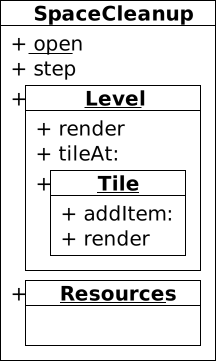
\includegraphics[scale=1]{nested_notation.pdf}
	\centering
	\caption{Nested Classes Example}
	\label{fig:concept_nested_notation}
\end{figure}

\section{Accessing the Lexical Scope}
It is sometimes necessary to access a method's outer lexical scope (i.e., the enclosing classes), in order to send messages to enclosing classes. Consider, for example, that we want to send a message \texttt{foo} to class \texttt{A B} within \texttt{A class>>B class>>C>>m5} in Figure~\ref{fig:concept_nested_notation}. Either one of the following two statements works in this case.

\begin{itemize}
	\item \texttt{A B foo.}
	\item \texttt{thisOuter foo.}
\end{itemize}

\texttt{thisOuter} is a keyword that evaluates to the method owner's enclosing class upon method compilation. Note, that \texttt{thisOuter} is bound to the method's lexical scope, not the receiver class' lexical scope.

\paragraph{Example}
Figure~\ref{fig:concept_lexical_thisouter} illustrates how \texttt{thisOuter} is bound. In \texttt{B1 class>>C class>>bar1}, \texttt{thisOuter} is bound to \texttt{B1}. In contrast, \texttt{B2 class>>C class>>bar2} binds \texttt{thisOuter} to \texttt{B2}. Consequently, \texttt{B1 C bar1} calls \texttt{B1 foo} and so does \texttt{B2 C bar1}, even though the receiver of \texttt{bar1} is an instance of \texttt{B2 C class} and not \texttt{B1 C class} in the latter case. Note, that \texttt{B2 C bar2} calls \texttt{B2 foo}, because \texttt{bar2}'s lexically enclosing class is \texttt{B2}.

\begin{figure}[!htp]
	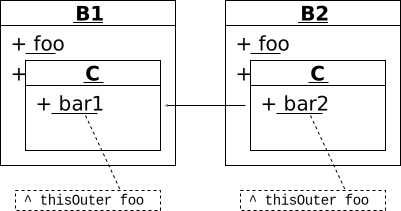
\includegraphics[scale=1]{nested_lexical1.pdf}
	\centering
	\caption{Binding of \texttt{thisOuter} to method's lexical scope.}
	\label{fig:concept_lexical_thisouter}
\end{figure}

thisOuter/thisContext keywords: send messages to lexical scope, all class references are late bound: always call accessor method, class aliasing

\section{Parameterized Classes}
mixins: functions from classes to classes
